\documentclass[11pt,reqno]{amsart}

\usepackage{amsmath,amssymb,graphicx,bbm}
\usepackage{amsthm,verbatim}
\usepackage{mathrsfs,mathtools,bm}

\usepackage[footnotesize,bf]{caption}
\usepackage[left=1.1in,right=1.1in,top=1in]{geometry}

\usepackage{graphicx}
\graphicspath{ {./images/} }

\pagenumbering{gobble}
\newcommand{\bs}[1]{\boldsymbol{#1}}
\newcommand{\mathd}{\textrm{d}}
\newcommand{\ddx}[1]{\frac{\mathd}{\mathd #1}}
\newcommand{\N}{\mathbbm{N}}
\newcommand{\R}{\mathbbm{R}}
\newcommand{\code}{\texttt}

%% Patch for amsart date
\usepackage{etoolbox}
\makeatletter
\patchcmd{\@maketitle}
  {\ifx\@empty\@dedicatory}
  {\ifx\@empty\@date \else {\vskip3ex \centering\footnotesize\@date\par\vskip1ex}\fi
   \ifx\@empty\@dedicatory}
  {}{}
\patchcmd{\@adminfootnotes}
  {\ifx\@empty\@date\else \@footnotetext{\@setdate}\fi}
  {}{}{}
\makeatother
%%

\title{Project 1: Finite difference methods}
\author{Preston Malen}
\date{February 2023}

\begin{document}
\maketitle

\noindent Consider the ordinary differential equation:
\begin{align}\label{eq:ode}
  \ddx{x} \left(\kappa(x) \ddx{x} u(x) \right) &= f(x), & x &\in [0,1],
\end{align}
with homogeneous Dirichlet boundary conditions, $u(0) = u(1) = 0$ , and where scalar diffusion coefficient $\kappa$ is given by,
  \begin{align*}
    \kappa(x) &= 2 + \sum_{\ell=1}^{5} \frac{1}{\ell+1} \sin( \ell \pi x ).
  \end{align*}
  The goal of this exercise will be to numerically compute solutions to this problem. \\[8pt]
  \begin{itemize}
    \item[(a)] Define the operator,
      \begin{align*}
        \widetilde{D}_0 u(x_j) &= \frac{u(x_j + h/2) - u(x_j - h/2)}{h}, & h &= 1/(N+1), & x_j &\coloneqq j h,
      \end{align*}
      for a fixed number of points $N \in \N$. Then with $u_j$ the numerical solution approximating $u(x_j)$ for solving the $d=1$ version of \eqref{eq:ode}, consider the scheme,
      \begin{align}\label{eq:D0-def}
        \widetilde{D}_0 \left( \kappa(x_j) \widetilde{D}_0 u_j \right) &= f(x_j), & j \in [N].
      \end{align}
      Show that, for smooth $u$ and $\kappa$, this scheme has second-order local truncation error.
    \item[(b)] Construct an exact solution via the \textit{method of manufactured solutions}: posit an exact (smooth) solution $u(x)$ (that satisfies the boundary conditions!) and, compute $f$ in \eqref{eq:ode} so that your posited solutions satisfies \eqref{eq:ode}.
    \item[(c)] Implement the scheme above for solving \eqref{eq:ode}, setting $f$ to be the function identified in part (b), so that you know the exact solution. Show that indeed you achieve second-order convergence in $h$ (say in the $h^{d/2}$-scaled vector $\ell^2$ norm) . (To ``show'' this, plot on a log scale the error as a function of a discretization parameter, such as $h$ or $N$, and verify that the slope of the resulting line is what is expected.)
  \end{itemize}
\newpage
\section*{\textbf{Solutions}}
\begin{itemize}
    \item[(a)] To calculate the local truncation error, we just need to expand the left-hand side of \eqref{eq:D0-def} and show we get a residual of $h^2$. So first, we consider the product $\kappa(x_j)\widetilde{D}_0u_j$:
    \begin{equation}\label{eq:arg}
        \kappa(x_j)\widetilde{D}_0u_j = \kappa(x_j)\bigg( \frac{u(x_j + h/2)-u(x_j -h/2)}{h}\bigg)
    \end{equation}
    Now, we apply the given difference operator $\widetilde{D}_0$ to \eqref{eq:arg}. For brevity, we will define the following:
    \begin{align*}
        \kappa_+ &= \kappa(x_j + h/2)\\
        \kappa_- &= \kappa(x_j - h/2)\\
        D_+ &= \kappa_+ \bigg( \frac{u(x_j + h) -u (x_j)}{h}\bigg)\\
        D_- &= \kappa_- \bigg( \frac{u(x_j) - u(x_j - h)}{h}\bigg)
    \end{align*}
    So in summary, we have the expression:
    \begin{equation}
        f(x_j) = \widetilde{D}_0 \left( \kappa(x_j) \widetilde{D}_0 u_j \right) = \frac{D_+ - D_-}{h}
    \end{equation}
    After some painful calculation, we get:
    \begin{equation*}
        h^2f(x_j) = -u(x_j)(k_+ + k_-) + k_+u(x_j + h) + k_-u(x_j-h)
    \end{equation*}
    So the given scheme does in fact have a local truncation error of $h^2$.\newline
    \\
    \item[(b)] Consider the function $u(x) = x(x-1)$. It is clear that $u$ has roots at $0$ and $1$ so the boundary conditions are satisfied. We will now compute $f(x)$ explicitly using the given parameters:
    %% NEED TO RE-CALCULATE/RE-WRITE EXACT SOLUTION
    \begin{align*}
        \ddx{x} \left(\kappa(x) \ddx{x} u(x) \right) &=  \ddx{x} \bigg[\bigg(2 + \sum_{\ell=1}^{5} \frac{1}{\ell+1} \sin( \ell \pi x )\bigg) \cdot (2x-1) \bigg]\\
        f(x) &= 4 +\sum_{\ell=1}^5 \frac{(2x-1)(\cos(\ell \pi x))(\ell \pi)+2\sin(\ell \pi x)}{\ell + 1}
    \end{align*}\newline
    \\
    \newpage
    \item[(c)] First, we choose a suitable $N$. For this problem, it was sufficient to choose $N \in [10^3,10^4]$ in increments of $10^3$. Graphed below, we have $N$ along the $x-$axis, and the local truncation error of the scheme on the $y-$axis. Note also that the local truncation error is graphed on a log scale.

    \begin{center}
        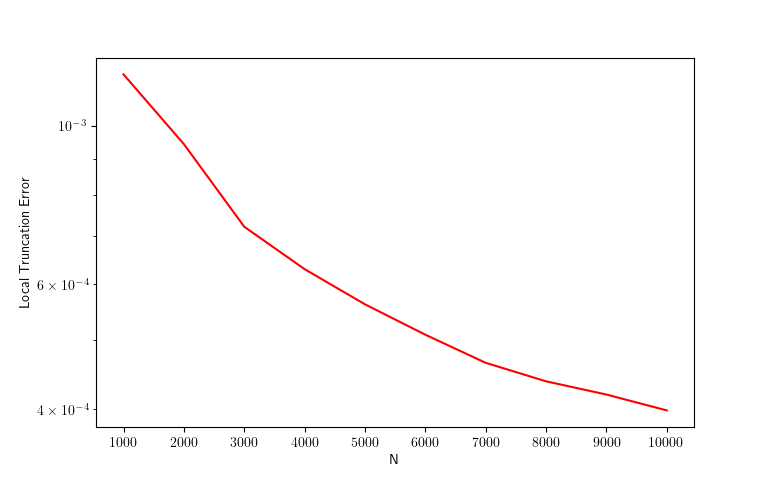
\includegraphics[scale=.7]{Figure_1.png}
    \end{center}\newline

    \noindent Using SciPy's \code{linalg} class, we found acceptable convergence and runtime using an iterative conjugate gradient method with default parameters. 
    
\end{itemize}

\end{document}
